\documentclass{article}

\usepackage{Sweave}
\begin{document}
\Sconcordance{concordance:accuracy_category.tex:accuracy_category.Rnw:%
1 2 1 1 0 45 1 1 23 3 0 1 1 9 0 1 17 2 0 1 1 9 0 1 21 2 0 1 1 9 0 1 19 %
2 0 1 1 10 0 1 2 2 1 1 8 1 3 2 1 1 7 1 3 5 1 1 6 1 3 3 1 1 6 1 3 3 1}


\title{Accuracy with latent categorical variable}

\author{Mc}
\maketitle
\section*{Introduction}
In plots we recast the results of simulations in terms of accuracy. We compute the accuracy of each method (continous or categorical), for each level of \(\rho\) (see below) by computing the  the following quantities:
\begin{itemize}
  \item false positive (FP)  runs with  with a significant test under a true null hypothesis
  \item true positive (TP) runs with a significant test under a false null-hypothesis 
  \item true negative (TN) runs  with a nonsignificant result under a true null-hypothesis
  \item false negative (FN) runs with a nonsignificant result under a false null-hypothesis

\end{itemize}

Plots to be produced:
\begin{itemize}
  \item Sensitivity for all 4 of the decision possibilities (continuous ignoring categorical, categorical ignoring continuous, both, either), with X axis being rho (Figure 1)
  \item PPV for the 4 decision possibilities, with X axis being rho (Figure 2)
  \item Bar chart with the specificity for the 4 decision possibilities
  \item Bar chart with the NPV (aggregated over rho) for the 4 decision possibilities
\end{itemize}

\section*{Setup}
\subsection*{Model}
A categorical latent variable ( \(\xi\) ) and a continuous one (\(\eta\) are created with N cases, sharing a correlation equal to \(\rho\). A measure \(x\) of \(\xi\) is created with reliability \(rel\), and then  is dichotomized accordingly to \(p\) \(1-p\) into \(c\). The correlations \( r_pe=r(\eta,x) \)  and \( r_pb=r(\eta,c) \) are computed, their p-value and significance (at .05) is recorded.
\subsection*{Design}
\(\rho=(0,.1,.2,.3,.4,.5,.6,.7) \)
\(rel=(0.3, 0.4 ,0.5, 0.6, 0.7 ,0.8 0.9) \) 


\subsection*{Computation of quantities}

\begin{itemize}
  \item Continuous false positive (FP\_C)  freq of runs with continuous test p.<.05 and \(\rho\)=0  
  \item Continuous true positive (TP\_C)  freq of runs with continuous test p.<.05 and \(\rho\) >0
  \item Continuous true negative (TN\_C) freq of runs  with continuous test p.>=.05 and \(\rho\)=0
  \item false negative (FN\_C)  freq of runs  with continuous test p.>=.05 and \(\rho\)>0
  \item PPV is defined as TP/(TP+FP)
  \item NPV is defined as TN/(TN+FN)
\end{itemize}

The same quantities are computed for the categorical indicator (*\_S).

\begin{Schunk}
\begin{Soutput}
Accuracy for continuous indicator
\end{Soutput}
\begin{Soutput}
  rho     SENS_C    SPEC_C       PPV       NPV
1 0.1 0.09957143 0.9497143 0.6644423 0.5133194
2 0.2 0.25342857 0.9497143 0.8344309 0.5598787
3 0.3 0.44314286 0.9497143 0.8980892 0.6303812
4 0.4 0.60228571 0.9497143 0.9229422 0.7048346
5 0.5 0.72042857 0.9497143 0.9347544 0.7725741
6 0.6 0.80942857 0.9497143 0.9415088 0.8328740
7 0.7 0.86457143 0.9497143 0.9450344 0.8751975
\end{Soutput}
\begin{Soutput}
Accuracy for categorical indicator
\end{Soutput}
\begin{Soutput}
  rho     SENS_S    SPEC_S       PPV       NPV
1 0.1 0.09857143 0.9491429 0.6596558 0.5128918
2 0.2 0.23714286 0.9491429 0.8234127 0.5544059
3 0.3 0.40400000 0.9491429 0.8881910 0.6142751
4 0.4 0.55128571 0.9491429 0.9155397 0.6789985
5 0.5 0.66071429 0.9491429 0.9285284 0.7366670
6 0.6 0.74485714 0.9491429 0.9360862 0.7881376
7 0.7 0.80385714 0.9491429 0.9404981 0.8287389
\end{Soutput}
\begin{Soutput}
Accuracy for BOTH indicators significant
\end{Soutput}
\begin{Soutput}
  rho     SENS_B    SPEC_B       PPV       NPV
1 0.1 0.06114286 0.9771429 0.7278912 0.5099911
2 0.2 0.17800000 0.9771429 0.8862020 0.5431158
3 0.3 0.35200000 0.9771429 0.9390244 0.6012658
4 0.4 0.50814286 0.9771429 0.9569545 0.6651755
5 0.5 0.62814286 0.9771429 0.9648892 0.7243461
6 0.6 0.72214286 0.9771429 0.9693193 0.7785999
7 0.7 0.78971429 0.9771429 0.9718706 0.8229066
\end{Soutput}
\begin{Soutput}
Accuracy for EITHER indicators significant
\end{Soutput}
\begin{Soutput}
  rho    SENS_E    SPEC_E       PPV       NPV
1 0.1 0.1370000 0.9217143 0.6363636 0.5164492
2 0.2 0.3125714 0.9217143 0.7997076 0.5727983
3 0.3 0.4951429 0.9217143 0.8634778 0.6461045
4 0.4 0.6454286 0.9217143 0.8918279 0.7221849
5 0.5 0.7530000 0.9217143 0.9058257 0.7886566
6 0.6 0.8321429 0.9217143 0.9140122 0.8459420
7 0.7 0.8787143 0.9217143 0.9181967 0.8837146
\end{Soutput}
\end{Schunk}

\subsubsection*{Figure 1: Sensitivity for all 4 of the decision possibilities (continuous ignoring categorical, categorical ignoring continuous, both, either), with X axis being rho}

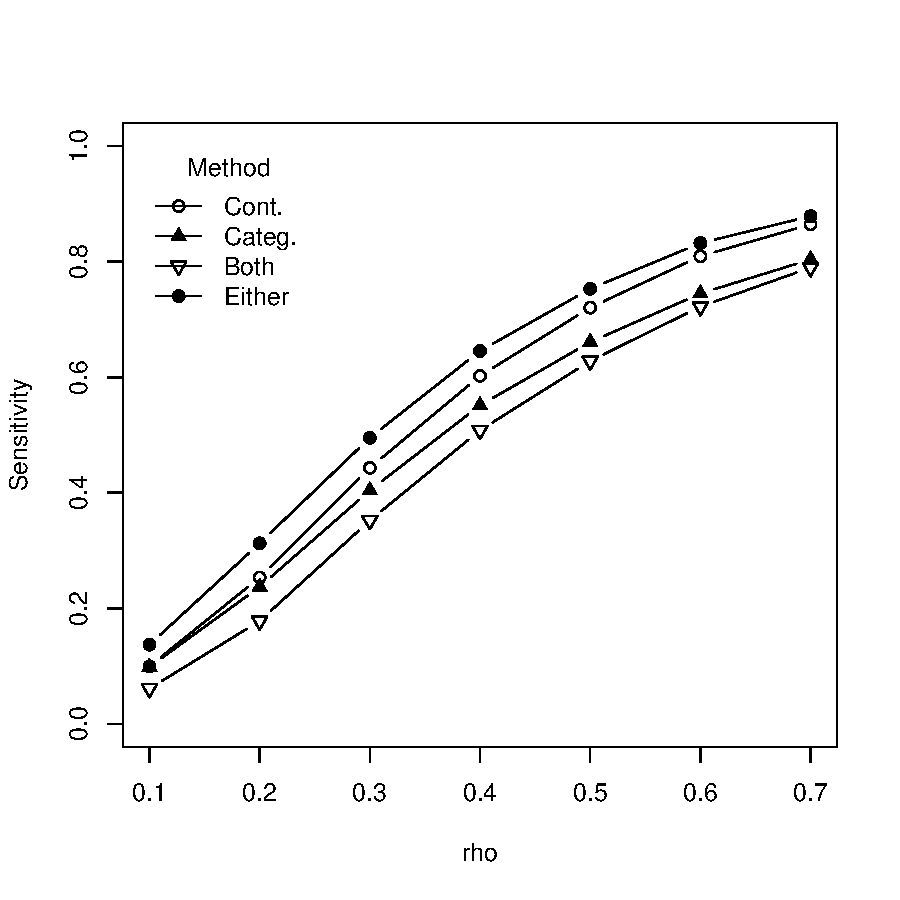
\includegraphics{accuracy_category-dd}

\subsubsection*{Figure 2: PPV for the 4 decision possibilities, with X axis being rho}

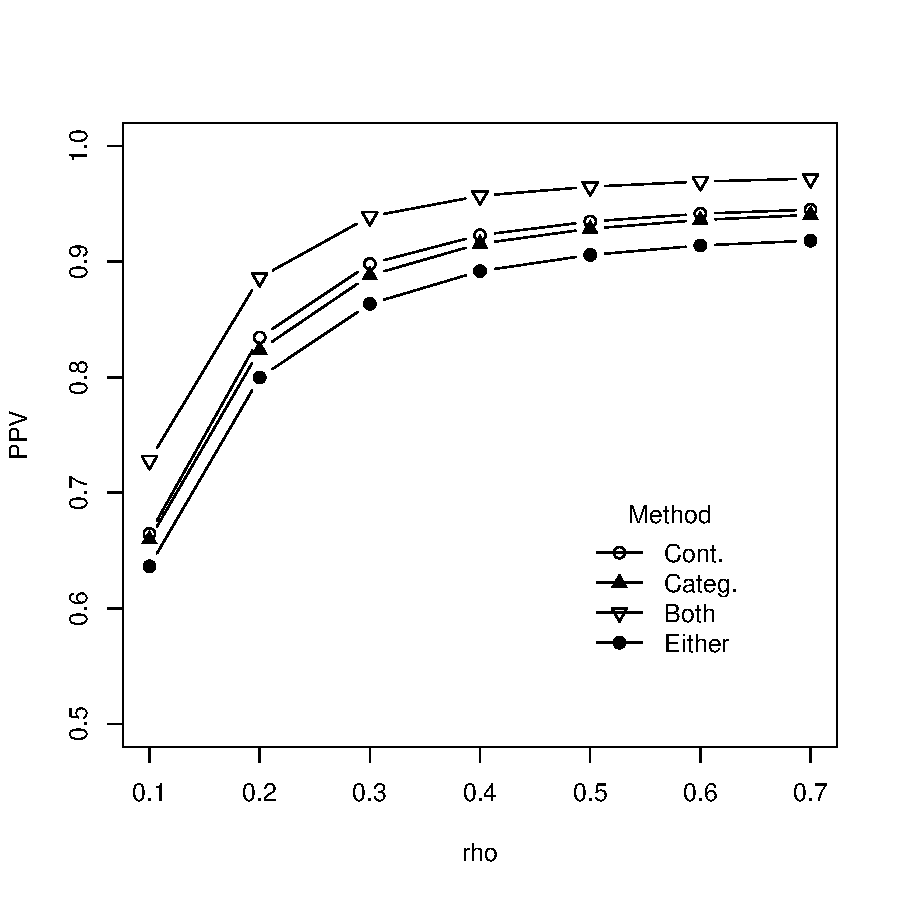
\includegraphics{accuracy_category-ee}


\subsubsection*{Figure 3: Bar chart with the specificity for the 4 decision possibilities }



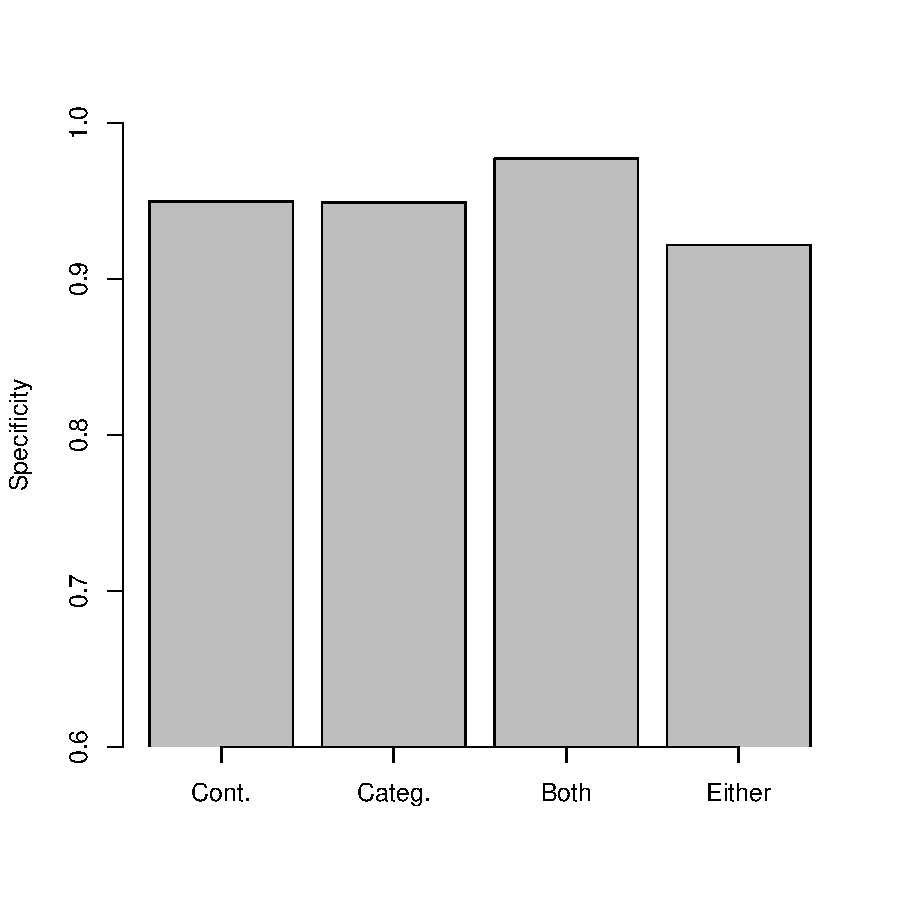
\includegraphics{accuracy_category-ff}

\subsubsection*{Figure 4: NPV for the 4 decision possibilities, with X axis being rho}


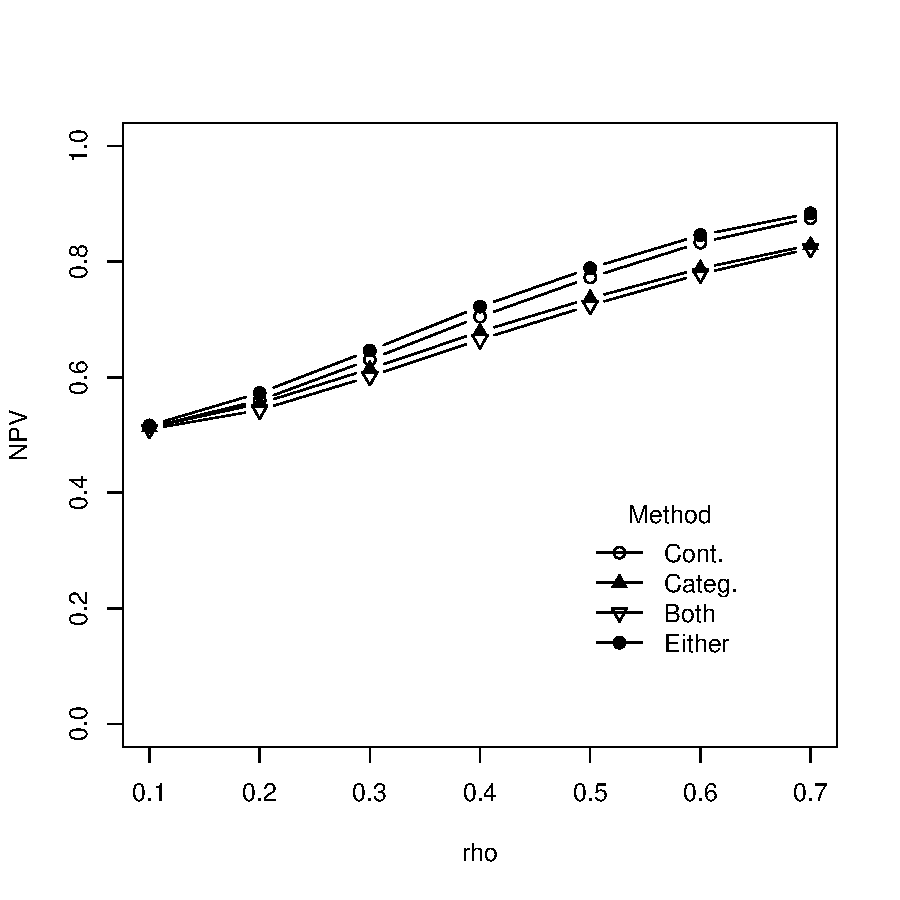
\includegraphics{accuracy_category-gg}



\end{document}
